%----------------------------------------------------------------------------------------
%	PACKAGES AND OTHER DOCUMENT CONFIGURATIONS
%----------------------------------------------------------------------------------------

\documentclass{tei2013}

\usepackage{times}
\usepackage{url}
\usepackage{graphics}
\usepackage{color}
\usepackage[pdftex]{hyperref}
\hypersetup{%
pdftitle={SceneCreator},
pdfauthor={Christine Talbot, Kenneth Hall, YongKang Liu, and Grace Christenbery},
pdfkeywords={Scenes, Surface, ImaginOn, ClipArt, Application},
bookmarksnumbered,
pdfstartview={FitH},
colorlinks,
citecolor=black,
filecolor=black,
linkcolor=black,
urlcolor=black,
breaklinks=true,
}
\newcommand{\comment}[1]{}
\definecolor{Orange}{rgb}{1,0.5,0}
\newcommand{\todo}[1]{\textsf{\textbf{\textcolor{Orange}{[[#1]]}}}}

%\pagenumbering{arabic}  % Arabic page numbers for submission.  Remove this line to eliminate page numbers for the camera ready copy

\usepackage{balance}
\usepackage{graphicx}
\usepackage[center]{caption}
\DeclareCaptionType{copyrightbox}
\usepackage{subcaption}
\usepackage{pdflscape}
\usepackage{rotating}

\usepackage{array}% http://ctan.org/pkg/array
 
\newcolumntype{C}{>{\centering\arraybackslash} m{.25\textwidth} }  %# New column type

\newcommand*{\plogo}{
\begin{subfigure}{.98\textwidth}
\centering
\includegraphics[width=.75\textwidth]{imgs/userstudy2}
\end{subfigure}
}

%----------------------------------------------------------------------------------------
%	TITLE PAGE
%----------------------------------------------------------------------------------------

\newcommand*{\titleGP}{\begingroup % Create the command for including the title page in the document
\centering % Center all text
\vspace*{\baselineskip} % White space at the top of the page

\rule{\textwidth}{1.6pt}\vspace*{-\baselineskip}\vspace*{2pt} % Thick horizontal line
\rule{\textwidth}{0.4pt}\\[\baselineskip] % Thin horizontal line

{\LARGE SceneCreator Project Report}\\[0.2\baselineskip] % Title

\rule{\textwidth}{0.4pt}\vspace*{-\baselineskip}\vspace{3.2pt} % Thin horizontal line
\rule{\textwidth}{1.6pt}\\[\baselineskip] % Thick horizontal line

\scshape % Small caps
Application Design and Evaluation \\[\baselineskip] % Tagline(s) or further description
April 26, 2013\par % Location and year

\vspace*{2\baselineskip} % Whitespace between location/year and editors
\vspace{45pt}
\plogo \\
\vspace{45pt}
Edited by \\[\baselineskip]
{\Large CHRISTINE TALBOT\\KENNETH HALL\\YONGKANG LIU\\GRACE CHRISTENBERY\par} % Editor list
\vspace{20pt}
{\itshape The University of North Carolina at Charlotte\par} % Editor affiliation
\vspace{70pt}
\vfill % Whitespace between editor names and publisher logo

%\plogo \\[0.3\baselineskip] % Publisher logo
%{\scshape 2012} \\[0.3\baselineskip] % Year published
{\large TANGIBLE DESIGN STUDIO}\par % Publisher

\endgroup}
%----------------------------------------------------------------------------------------
%	BEGIN DOCUMENT - TITLE PAGE
%----------------------------------------------------------------------------------------

\begin{document} 
\pagestyle{empty} % Removes page numbers
\begin{figure*}[h]
\titleGP
\end{figure*}
%\titleGP % This command includes the title page
\clearpage
\pagebreak

\balance

%%----------------------------------------------------------------------------------------
%%	TITLE INFO
%%----------------------------------------------------------------------------------------
%
%
%\title{Photo Menagerie}
%\numberofauthors{1}
%\author{
%\alignauthor
%Christine Talbot, Kenneth Hall, YongKang Liu, and Grace Christenbery\\
%\affaddr{Tangible Design Studio}\\
%\affaddr{University of North Carolina at Charlotte}\\
%\email{\{ctalbot1, kdhall1, lyongkan, gchriste\}@uncc.edu}
%}
%
%%----------------------------------------------------------------------------------------
%%	BEGIN DOCUMENT
%%----------------------------------------------------------------------------------------
%
%\begin{document} 
%
%\maketitle

%----------------------------------------------------------------------------------------
%	ABSTRACT
%----------------------------------------------------------------------------------------
%\begin{abstract}
%ABSTRACT OF PAPER - short version of Introduction\\
%
%\end{abstract}

%\keywords{Collage, Surface, Museum, Photos, Application}
%
%\category{H.5.2}{Information Interfaces and Presentation}{Miscellaneous}
%
%\subsection{General Terms}
%Design, Experimentation, Human Factors

\balance
%----------------------------------------------------------------------------------------
%	INTRODUCTION
%----------------------------------------------------------------------------------------
\section{Introduction}
\textcolor{red}{1.	Title page\\
2.	Description of the purpose of the application\\
3.	User and stakeholder groups (types)\\
4.	Results of user studies to generate user needs and desires\\
5.	Description of working prototype including system architecture and interaction design\\
6.	User evaluation of working prototype\\
7.	Evaluation of the use of gesture and tangible interaction\\
8.	CD with all working code and installation instructions
}
%\subsection{Yongkang}
%What is the paper about?  Application Purpose, Overview of the paper outline \& findings teaser
Tangible interaction with digital models changes our perception of the design model. The tangible application development processes are different from the traditional computer application design processes. In this article, we introduce some research works on tangible user interface design and the relationships between gestures and human cognition, such as Casasanto and Lozano's work ``The meaning of metaphorical gestures" \cite{Casasanto_MG2008_MeaningOfMetaphoricalGestures} and Cienki and M\"{u}ller's work ``Metaphor, gesture, and thought" \cite{Cienki_CHMT2008_MetaphorGestureThought}.

We developed Photo Menagerie  application to practise the design methods for tangible devices. Photo Menagerie is a application placed on the Microsoft PixelSense Surface device in a museum or public area for visitors to share pictures and create collages from those pictures. Pictures are expected to be from the visit at the museum. Users can work together or individually to create a collage. The collages may be printable in an 8"x11" black and white format, or in full color poster size in the gift shop. Images and collages collected by the system can be utilized by the museum administration to create their own posters or marketing materials.

We used personas and prototype design methods to develop application features.  The personas are a user centered design approach, which is useful in collecting requirements.  The prototype design is a fast iterative design approach to get feedback from end users.
%We used personas and prototype design methods to develop application features. The personas is a user centered design approach, which is useful in collecting requirements. The prototype design is a fast iterative design approach to get feedback from end users. 
We evaluated the application's usage by doing gesture and action analysis that checks if gestures are consistent with actions.
%----------------------------------------------------------------------------------------
%	PURPOSE
%----------------------------------------------------------------------------------------
\section{Related Work}
The application will be placed on the Microsoft PixelSense Surface device in a museum or public area for visitors to share pictures and create collages from those pictures.  Pictures are expected to be from the visit at the museum.  Users can work together or individually to create a collage.  The collages may be printable in an 8x11” black and white format, or in full color poster size in the gift shop.  Images and collages collected by the system can be utilized by the museum administration to create their own posters or marketing materials.

%----------------------------------------------------------------------------------------
%	STAKEHOLDERS
%---------------------------------------------------------------------------------------
\section{Stakeholders}

\subsection{Museum Administrators}
The expected stakeholders are museum administrators and application supporters.
As museum administrators, they want to sell posters and marketing materials.
As application supporters, they want to upgrade the application and change the application user interfaces or desktop themes.%----------------------------------------------------------------------------------------
%	USERS
%---------------------------------------------------------------------------------------
\section{Users}
The users are varied and may include children, teenagers, young adults, middle aged adults, and senior citizens. Most people that travel through the museum will have interest in what the museum has to offer and will use the application we are building to remember the visit. 
\subsection{Academic Groups}
This group includes students attending the museum as a field trip with their school for learning and fun.  Teachers may utilize the tabletop for creative outlet for the children, and provide photo devices for taking pictures.  Children may use it to print out their memories of the trip in a collage in black and white, or send it to their parents for printing / buying later.
\subsection{Families}
This group is very similar to the academic groups, but will look to print out family related pictures and experiences as a whole.  They may include younger children than the academic groups, however the expectation is that the parents will drive or supervise most of the interaction with the device.  
\subsection{General Public}
The users may also include groups of friends who wish to spend time at the museum for social reasons.  They may share their images with friends and family on social sites such as Facebook.
\subsection{Enthusiasts}
Group of people with a common interest geared towards learning and discovering more about the museum's subject area (art, science, and so forth).  These people may focus on images of the museum's artifacts more than people within the museum.


%----------------------------------------------------------------------------------------
%	APPROACH
%----------------------------------------------------------------------------------------
\section{Approach}
%\subsection{Kenneth}
For our approach on the Photo Menagerie project, we applied sever design methods to create multiple prototypes. Each of us created our own type of soft prototypes to contribute ideas, then we as a group went over them and decided which features were the best for the overall project. 

Using these methods, we created a paper prototype with paper pieces that enable Wizard of Oz testing, another paper prototype that is based on several drawn pictures, and a digital drawing (paper) prototype. After deciding on features, we changed the primary paper prototype to look similar to the idea we created, implementing all of the new features. 

With this new paper prototype, we conducted several user studies. Taking it into a lab environment, we asked individuals to test it out as if they were an actual user. As they interacted with it, they thought aloud as we played the role of the Wizard of Oz, exchanging pieces out. We made notes of complications, successes, and a final overview of the user's experience. 

We also developed a list of personas to help us design towards. Our targeted audience is a very general range of people, from children and school groups, to teenagers, adults, and enthusiasts. Therefore, we had a broad range of personas. 

%----------------------------------------------------------------------------------------
%	USER-CENTERED DESIGN METHODS
%---------------------------------------------------------------------------------------
\section{User-Centered Design Methods}
We utilized two user-centered design methods to assist with designing our application.
\subsection{Participant Observation}
This method requires us to observe users using either our system or a similar system.  We observed two users using the Photovisi application online which allows users to upload their photos and create a collage with them.  These collages can then be emailed, shared on facebook, or put onto merchandise.  This is very similar to the kind of usage we expect to have with our application within the museum.  Some key findings from this process included:
\begin{itemize}\itemsep0em
\item{Has large buttons that make it clear what can be done}
\item{The active picture can be scaled, rotated, translated, or skewed}
\item{Some of the templates are too complex and are frustrating to move around those details}
\item{Was not clear on how many photos were needed until after selected photos}
\item{Layering is not obvious, but did have buttons on the side if you can get to the photo}
\item{Download options are not clear}
\end{itemize}
%Describe what did - anthropological approcah to observe how users use it \& make iterative refinements
%Look at PhotoGrid and PicStitch and Photovisi \& have one of us use it and take notes
\subsection{Personas}
We created fictional characters for each of the user groups described above and discussed their desired goals and pain points.  We named them:
\begin{description}\itemsep-.5pt
\item[Teacher]{Tom Ryan - 4th grade teacher challenged to encourage sharing}
\item[Student]{Sally Crocker - shy 4th grader who wants to be creative}
\item[Parent]{Jan Davis - mother of two who wants to share her trip with family}
\item[General Public]{John Q. Citizen - broke tourist visiting from Seattle}
\item[Enthusiast]{Arty Decker - art collector who wants self-created custom framed art}
\item[Museum Administrator]{Marissa Curie - museum administrator of 11 years who wants the profits to exceed the cost of the device}
\end{description}


%\subsection{Methods}
%----------------------------------------------------------------------------------------
%	THREE SOFT PROTOTYPES
%---------------------------------------------------------------------------------------
\subsection{Soft Prototypes}
Three different approaches were pursued for prototyping the application.  The first is a windows-based approach with one session on the table at a time.  The second one is a state-based approach also covering the entire table for a single session.  The third prototype is an interactive two-session approach on the single table.  In the following sections, each approach is described and sketched.

%----------------------------------------------------------------------------------------
%	Prototype #1
%---------------------------------------------------------------------------------------
\subsubsection{Prototype \#1}
Prototype \#1 is the design that allow users to import pictures and create collages. The prototype seen in Figure~\ref{fig:prot1} demonstrates the actions that users can perform on the table. 
\begin{figure}[h]
\centering
\fbox{\includegraphics[width=.48\textwidth]{imgs/prototype1}}
\caption{Prototype \#1 Image}
\label{fig:prot1}
\end{figure}

Prototype \#1 supports multiple users at the same time. And it has following functions for users. At the beginning, users import and delete pictures within the interface. Then users create a new collage and choose a frame. Users can add and remove pictures in the collage. All pictures and collages can be rotated and zoomed. At the end, users print the collage.

From gesture perspective, the surface supports touch and move gestures. After insert camera memory cards into the surface device, users touch ``Add photo" to select the pictures from the window explorer. The pictures appear in the Figure~\ref{fig:prototype1-1}. And users can delete the pictures from the pop-up menu (See Figure~\ref{fig:prototype1-2}). Touch empty area in the table and choose ``Add new" from the menu to create a new Collage (See Figure~\ref{fig:prototype1-3}). Users can move the slide bar to choose a collage frame(See Figure~\ref{fig:prototype1-4}). In order to add the pictures into the collage, touch and move pictures (See Figure~\ref{fig:prototype1-5}). The surface supports multiple fingers and users can use two fingers to rotate and zoom the collages and pictures (See Figure~\ref{fig:prototype1-6}). Touch empty area in the collage to choose ``Export" from the menu to print the collage (See Figure~\ref{fig:prototype1-7}).
\begin{figure*}[htb]
\centering
\begin{subfigure}[b]{.24\textwidth}
\centering
\fbox{\includegraphics[width=\textwidth, height=100pt]{imgs/prototype1-1}}
\caption{Import Pictures}
\label{fig:prototype1-1}
\end{subfigure}
\begin{subfigure}[b]{.24\textwidth}
\centering
\fbox{\includegraphics[width=\textwidth, height=100pt]{imgs/prototype1-2}}
\caption{Delete Pictures}
\label{fig:prototype1-2}
\end{subfigure}
\begin{subfigure}[b]{.24\textwidth}
\centering
\fbox{\includegraphics[width=\textwidth, height=100pt]{imgs/prototype1-3}}
\caption{Add a New Collage}
\label{fig:prototype1-3}
\end{subfigure}
\begin{subfigure}[b]{.24\textwidth}
\centering
\fbox{\includegraphics[width=\textwidth, height=100pt]{imgs/prototype1-4}}
\caption{Choose a Frame}
\label{fig:prototype1-4}
\end{subfigure}
\begin{subfigure}[b]{.24\textwidth}
\centering
\fbox{\includegraphics[width=\textwidth, height=100pt]{imgs/prototype1-5}}
\caption{Add Pictures to the Collage}
\label{fig:prototype1-5}
\end{subfigure}
\begin{subfigure}[b]{.24\textwidth}
\centering
\fbox{\includegraphics[width=\textwidth, height=100pt]{imgs/prototype1-6}}
\caption{Rotate and Zoom}
\label{fig:prototype1-6}
\end{subfigure}
\begin{subfigure}[b]{.24\textwidth}
\centering
\fbox{\includegraphics[width=\textwidth, height=100pt]{imgs/prototype1-7}}
\caption{Print the Collage}
\label{fig:prototype1-7}
\end{subfigure}

\caption{Prototype \#1 Actions}
\end{figure*}

%----------------------------------------------------------------------------------------
%	Prototype #2
%---------------------------------------------------------------------------------------
\subsubsection{Prototype \#2}
Prototype \#2 is a design based on a more simplistic approach. It is catered to a single user, therefore taking up the entire screen. Other designs featured multiple users on the same surface, but this one featured the entire interface being for one user. 
\begin{figure*}[htb]
\centering
\begin{subfigure}[b]{.48\textwidth}
\centering
\fbox{\includegraphics[width=\textwidth, height=170pt]{imgs/prototype2-1}}
\caption{Prototype \#2 Pictures Screen}
\label{fig:prot2-1}
\end{subfigure}
\begin{subfigure}[b]{.48\textwidth}
\centering
\fbox{\includegraphics[width=\textwidth, height=170pt]{imgs/prototype2-2}}
\caption{Prototype \#2 Layout Screen}
\label{fig:prot2-2}
\end{subfigure}

\caption{Prototype \#2 Sketches}
\end{figure*}

This paper prototype was based on using multiple layers of interaction within the interface. The first layer is the ``Picture" layer, as seen in Figure~\ref{fig:prot2-1}. In this layer the user can load their pictures. They select their device if it's bluetooth connected or if they used the card recognition feature throughout the museum, they may select those pictures. Also in the picture layer the user can select which pictures they want to add to their gallery, which is the bank of photos they'll use to make the collage. 

The next layer is the ``Layout" layer (seen in Figure~\ref{fig:prot2-2}), which allows the user to create their collage. The Layout layer first contains a set of templates in which the user can choose from. Upon choosing their desired template, the user can touch the "Next" button at the bottom right on the surafce. From there they can access their gallery of pictures and place pictures into desired spots in the collage. 

After the user achieves the desired collage look and layout, they can select the ``Finish" layer. In this layer the user can select what they would like to do with their collage. Some examples are getting prints in different sizes or posters, getting it printed on coffee mugs, mousepads, etc, or sharing the collage on a social network. 

This design, as seen in Figure~\ref{fig:prot2} entails a very simple structure in which the user follows a direction of interaction based on a set of layers. Active layers are visible while layers yet to be accessed are ghosted out. This method of user interaction helps for controlling the user's actions. It also allows the user to recognize progression and therefore is extremely intuitive while appearing to be fun, exciting and easy to use. 

%see Figure~\ref{fig:prot2}.
\begin{figure}[ht]
\centering
\fbox{\includegraphics[width=.48\textwidth]{imgs/prototype2}}
\caption{Prototype \#2 Image}
\label{fig:prot2}
\end{figure}

%----------------------------------------------------------------------------------------
%	Prototype #3
%---------------------------------------------------------------------------------------
\subsubsection{Prototype \#3}
This prototype attempts encourage more than one collage session on the table at a time.  To do this, the table is split in half, providing reasonable working space, but still allows users to feel like their pictures are theirs and no one else's.  It also assumes the ability to provide cameras within the museum and ``kodak" spots throughout the museum for visitors to capture pictures, even if they do not have a camera, camera phone, or other photo-taking device with them.  A paper mockup can be seen in Figure~\ref{fig:prot3-paper}.

To better describe this prototype, we will refer to the Storyboard in Figure~\ref{fig:story3}.  To begin, visitors are provided a unique key (including a clip) with a specific barcode on it to utilize during their visit.  They can swipe this key for the special ``kodak" spots to identify themselves and have pictures taken throughout the museum.  This key could also be used within a phone app to enable visitors to utilize their own photo-taking device and upload them for use with the application.
\begin{figure}[ht]
\centering
\fbox{\includegraphics[width=.48\textwidth]{imgs/prototype3-full}}%{prototype3-paper}}
\caption{Paper Mockup of Prototype \#3}
\label{fig:prot3-paper}.
\end{figure}
 
When the visitors finish their visit, they can choose to utilize the Photo Menagerie application on the surface table.  When no one is utilizing the table (either side or both sides), a screen-capture video of putting together a collage will play, exposing just the two ``place key here" locations on the table.  The text on the ``place key her" locations will be on all four sides of the box, each one with a different orientation of the text to encourage usage from any direction.

Once the key is placed on the table, the application will appear on that side of the table, with the same orientation as the key's placement.  A sample of what the application will look like can be seen in Figure~\ref{fig:prot3}.  In the center is an empty box with a bar on each edge that says ``TOP", with one of them being highlighted in red to indicate the current top.  The default selection for the red TOP bar will be based on the key's orientation when placed on the table, but can be changed at any time by tapping one of the TOP bars, or re-orienting the key.  Also on this TOP bar will be the standard iOS SendTo icon (a box with an arced arrow) to support the different print options.

Below this box will be a picture viewer, sort of like what Macintosh users see when viewing folders of pictures on their machine.  The middle image will be the largest and in front, with the slider on the bottom allowing the user to scroll through all the images they took using their key.  The scroller will help the users to understand where they are in their pile of pictures while reviewing them.  The orientation of the pictures will be based on the key's orientation as well, to ensure appropriate visibility to the user.  No zooming is allowed in this part of the application.

All around the collage box will be different options for the picture layout templates.  These templates will be mirror-reflected down the long centerline of the table when looking at both halves of the table together.  This will ensure all the templates are available on any half-division of the table for the users.  Lining the borders with the templates also helps to delineate the two different instances of the application on the table for the users.
\begin{figure*}[htb]
\centering
\begin{subfigure}[b]{.48\textwidth}
\centering
\fbox{\includegraphics[width=\textwidth, height=170pt]{imgs/storyboard3}}
\caption{Prototype \#3 Storyboard}
\label{fig:story3}
\end{subfigure}
\begin{subfigure}[b]{.48\textwidth}
\centering
\fbox{\includegraphics[width=\textwidth, height=170pt]{imgs/prototype3}}
\caption{Prototype \#3 Image}
\label{fig:prot3}
\end{subfigure}

\caption{Prototype \#3 Sketches}
\end{figure*}

To choose a template, the user(s) can drag the one they like to the collage box.  The lines of the template can slide along the line's perpendicular to allow for a different ratio of the width or length of the collage for each section.  The template itself can also be double-tapped to open a color / pattern selector for the outer template area, and may include stripes, confetti, solid colors, and the like.

Once the template is selected, the user(s) can drag the photos they like into the slots provided by the template.  Once in place, the photo can be enlarged or shrunk utilizing a pinch motion on the photo, or can be rotated and slid with the typical motions for these actions.  If the user places a second photo on top of a slot that already has a photo, the first photo will be returned to the photo deck.  Photos can be reused more than once / in multiple slots on the template.  They will always be placed underneath the template and if the edges of the photo lie outside its slot on the template, those excess parts will not be visible.  There will also be an auto-button next to the picture slider to allow the system to auto-select a default template and randomly place the right number of pictures into the template for the user.

When the user is finished, they can touch the iOS SendTo icon on the TOP bar to see their choices for printing.  It will show a menu of images for: black and white 8 1/2" x 11" printout (limit one per key), full color poster printout of any size from gift shop, T-shirt print in gift shop, cup print in gift shop, or email to self with a watermark.  Multiple gift shop selections can be made and saved into a shopping cart.  Once submitted, the user can retrieve the black and white printout below the table, or the gift shop items from the gift shop after the designated time from the application.  

If the user removes their key card, the application will clear itself and return to idle mode (video playing).  If the same key card is placed on the table again, it will show wherever the user left off previously.\\


%----------------------------------------------------------------------------------------
%	USER STUDIES
%---------------------------------------------------------------------------------------
\subsection{User Studies}
Two user studies were performed with different user groups to assist with analyzing the differing approaches from the different prototypes described above.  Each study is described in the below sections, along with some of the key observations made.

%Describe briefly how the user studies were performed, along with how many (at least 2)
%----------------------------------------------------------------------------------------
%	USER STUDY #1
%---------------------------------------------------------------------------------------
\subsubsection{User Study \#1}
The Future Computing Lab (FCL) researchers, a group of five people (seen in Figure~\ref{fig:user1}), performed a user test on our paper prototype as we used the Wizard of Oz method. We sat the initial design there and let the user work with it without our assistance. As the user selected options, we would change the layout accordingly, essentially as the application is designed to perform. 
\begin{figure}[ht]
\centering
\fbox{\includegraphics[width=.48\textwidth]{imgs/userstudy1}}
\caption{FCL Researcher Utilizing the Prototypes}
\label{fig:user1}
\end{figure}

While the primary user performed operations within the ``application" the others made comments and suggestions about how to use the system. For the most part, the system was intuitive, but the low fidelity did create difficulties in understanding certain functions. 

During the use of the system, users made comments about improvements and functionality we had not already addressed, which was helpful. The users pointed out flaws and generated feedback on the overall use of the application. We then developed a list of many functions that we can implement to make our system better. 

Some suggestions and thoughts which were verbalized included:
\begin{itemize}
\item The testers of the prototype suggested that when you hit ``Done" that there should be an indication or warning of some kind to quit or exit. 
\item Users like the ability to select photos, which then added the selected ones to the ``gallery", rather than dragging the undesired pictures to the ``trash" icon.
\item Users did not like the inability to retrieve accidentally deleted pictures from the trash. This is solved by using a picture selection and adding to the gallery.
\item Users are curious about saving their state. This is automatic, in case the key is accidentally removed, allowing for the user to be able to edit something then come back to finish it later. 
\item More control around stages / layers looked nicer according to the users. 
\item Users desired the ability to share across the table by flicking a picture across, thus allowing for multiple users to interact with each other and exchange photos. 
\item Having the ability to add lines to the templates, thus creating their own template was an additional desire for users. 
\item The ability to slide the lines around on the templates to adjust picture space was asked for by the testers. 
\item The users wanted to be able to decipher between dragging the icons or not in order to utilize its functionality, versus only touching them. 
\item The users did not attempt to zoom or reorient the pictures, but it must still be considered for future testing. 
\item The users did not ask about moving or reorienting the key, which will change the orientation of their workspace. 
\item If the user accidentally hit done, then their sessions ends, therefore the users proposed that we develop a method to get back to the session. 
\item The users asked about scrolling on pictures.
\item It was also asked if they could add text to the images.
%
%\item Done - should say quit or exit, include warning message
%\item Liked select versus trash
%\item Can we retrieve from the trash? How undelete?
%\item Saving state
%\item More control around stages nicer
%\item Sharing across the table - flick to send pictures across
%\item Adding own lines to templates
%\item Sliding the lines on the templates
%\item Seeing the icons draggable or not versus touch only
%\item Didn't try to zoom or reorient pictures
%\item Didn't ask about removing the key or moving it / orientation
%\item If accidentally hit done - how get back to their session, is it possible?
%\item Asked about scrolling on pictures
%\item Asked if they could add text to the images
\end{itemize}

%Describe this user study (how performed, who, etc) and their response to the prototype -- include an image

%----------------------------------------------------------------------------------------
%	USER STUDY #2
%---------------------------------------------------------------------------------------
\subsubsection{User Study \#2}
The second user-study performed involved interviews of two different security specialists in the Cyber Corps lab at the University of North Carolina at Charlotte. Given limited context and preset ideas, each  interviewee was asked to creatively design from scratch what felt most ``intuitive" to them as a photo app. Context details were slowly revealed if deemed necessary through out the process. Furthermore, both interviewees revealed security flaws in the design of the app regarding personal privacy. The first interviewee, Antionette Parnther, is a Information Security specialist with a focus in privacy. The second interviewee, Michael Rosa, is an Information Security specialist and President of the 49th Security Division.

The interviewees suggested ideas that they would like to see in such an app, the ideas included the following:
\begin{itemize}
\item Silly features, such as adding things like emoticons and top hats or ``flipping the table" to make the photos fly off and restart, were requested by this group of users. 
\item Info tips for pictures taken in certain parts of the museum or about individual paintings.
\item Limited the features to streamline the process; assume the user does not want to wait his or her turn.
\item Paint by numbers option for outlines of paintings.
\item Painting effects on pictures make photos look like paintings.
\item No automatic picture taking, only use keys in designated photo-taking areas that only allow one person or group at a time to take pictures to prevent strangers from obtaining private photos.
\item Green screen effect to put you ``inside" a painting.
\item Use image icons rather than text for any menu item required.
\item The users desired the ability drag photos to a shopping cart to purchase print outs.
\item No personal details should ever to be entered on the Surface, the screen is large and the data could be compromised by other visitors; instead, purchase requests for prints are sent to the physical store.
\item Black is the best choice for a background color opposed to a texture due to color theory; colors appear different when placed next to different colors or textures and in an art experience this effect is unwanted.
%\item Silly features, adding things like emoticons and tophats or ``flipping the table" to make the photos fly off and restart
%\item Info tips for pictures taken in certain parts of the museum or about individual paintings
%\item Limited features to streamline the process, assume the user does not want to wait his or her turn
%\item Paint by numbers option for outlines of paintings
%\item Painting effects on pictures, make photos look like paintings
%\item No automatic picture taking, only use keys in designated photo-taking areas that only allow one person or group at a time to take pictures to prevent strangers from obtaining private photos
%\item Green screen effect to put you ``inside" a painting
%\item Use image icons rather than text for any menu items required
%\item Drag photos to a shopping cart to purchase print outs
%\item No personal details are ever to be entered on the Surface, the screen is large and the data could be compromised by other visitors; instead, purchase requests for prints are sent to the physical store
%\item Black is the best choice for a background color opposed to a texture due to color theory; colors appear different when placed next to different colors or textures and in an art experience this effect is unwanted
\end{itemize}

\begin{figure}[ht]
\centering
\fbox{\includegraphics[width=.48\textwidth]{imgs/userstudy2}}
\caption{A Design by a Security Specialist Interviewee of an Intuitive, Secure User-Interface}
\label{fig:user1}
\end{figure}

When asked how each interviewee would use the app, one response was mainly for purchasing silly photos or actual copies of paintings in the museum. The second response was to purchase photos for sentimental value; both responses emphasized purchasing photos, simplicity, and speed rather than creative expression.
\begin{figure*}[Ht]
\centering
\begin{subfigure}[b]{.48\textwidth}
\centering
\fbox{\includegraphics[width=\textwidth, height=120pt]{imgs/merged-picsstate}}
\caption{Photo Review Screen Triggered by a User Key}
\label{fig:finalpic}
\end{subfigure}
\begin{subfigure}[b]{.48\textwidth}
\centering
\fbox{\includegraphics[width=\textwidth, height=120pt]{imgs/merged-layoutstate}}
\caption{Layout Design Screen}
\label{fig:finallayout}
\end{subfigure}
\begin{subfigure}[b]{.48\textwidth}
\centering
\fbox{\includegraphics[width=\textwidth, height=120pt]{imgs/merged-finishstate}}
\caption{Printing Screen}
\label{fig:finalfinish}
\end{subfigure}
\begin{subfigure}[b]{.48\textwidth}
\centering
\fbox{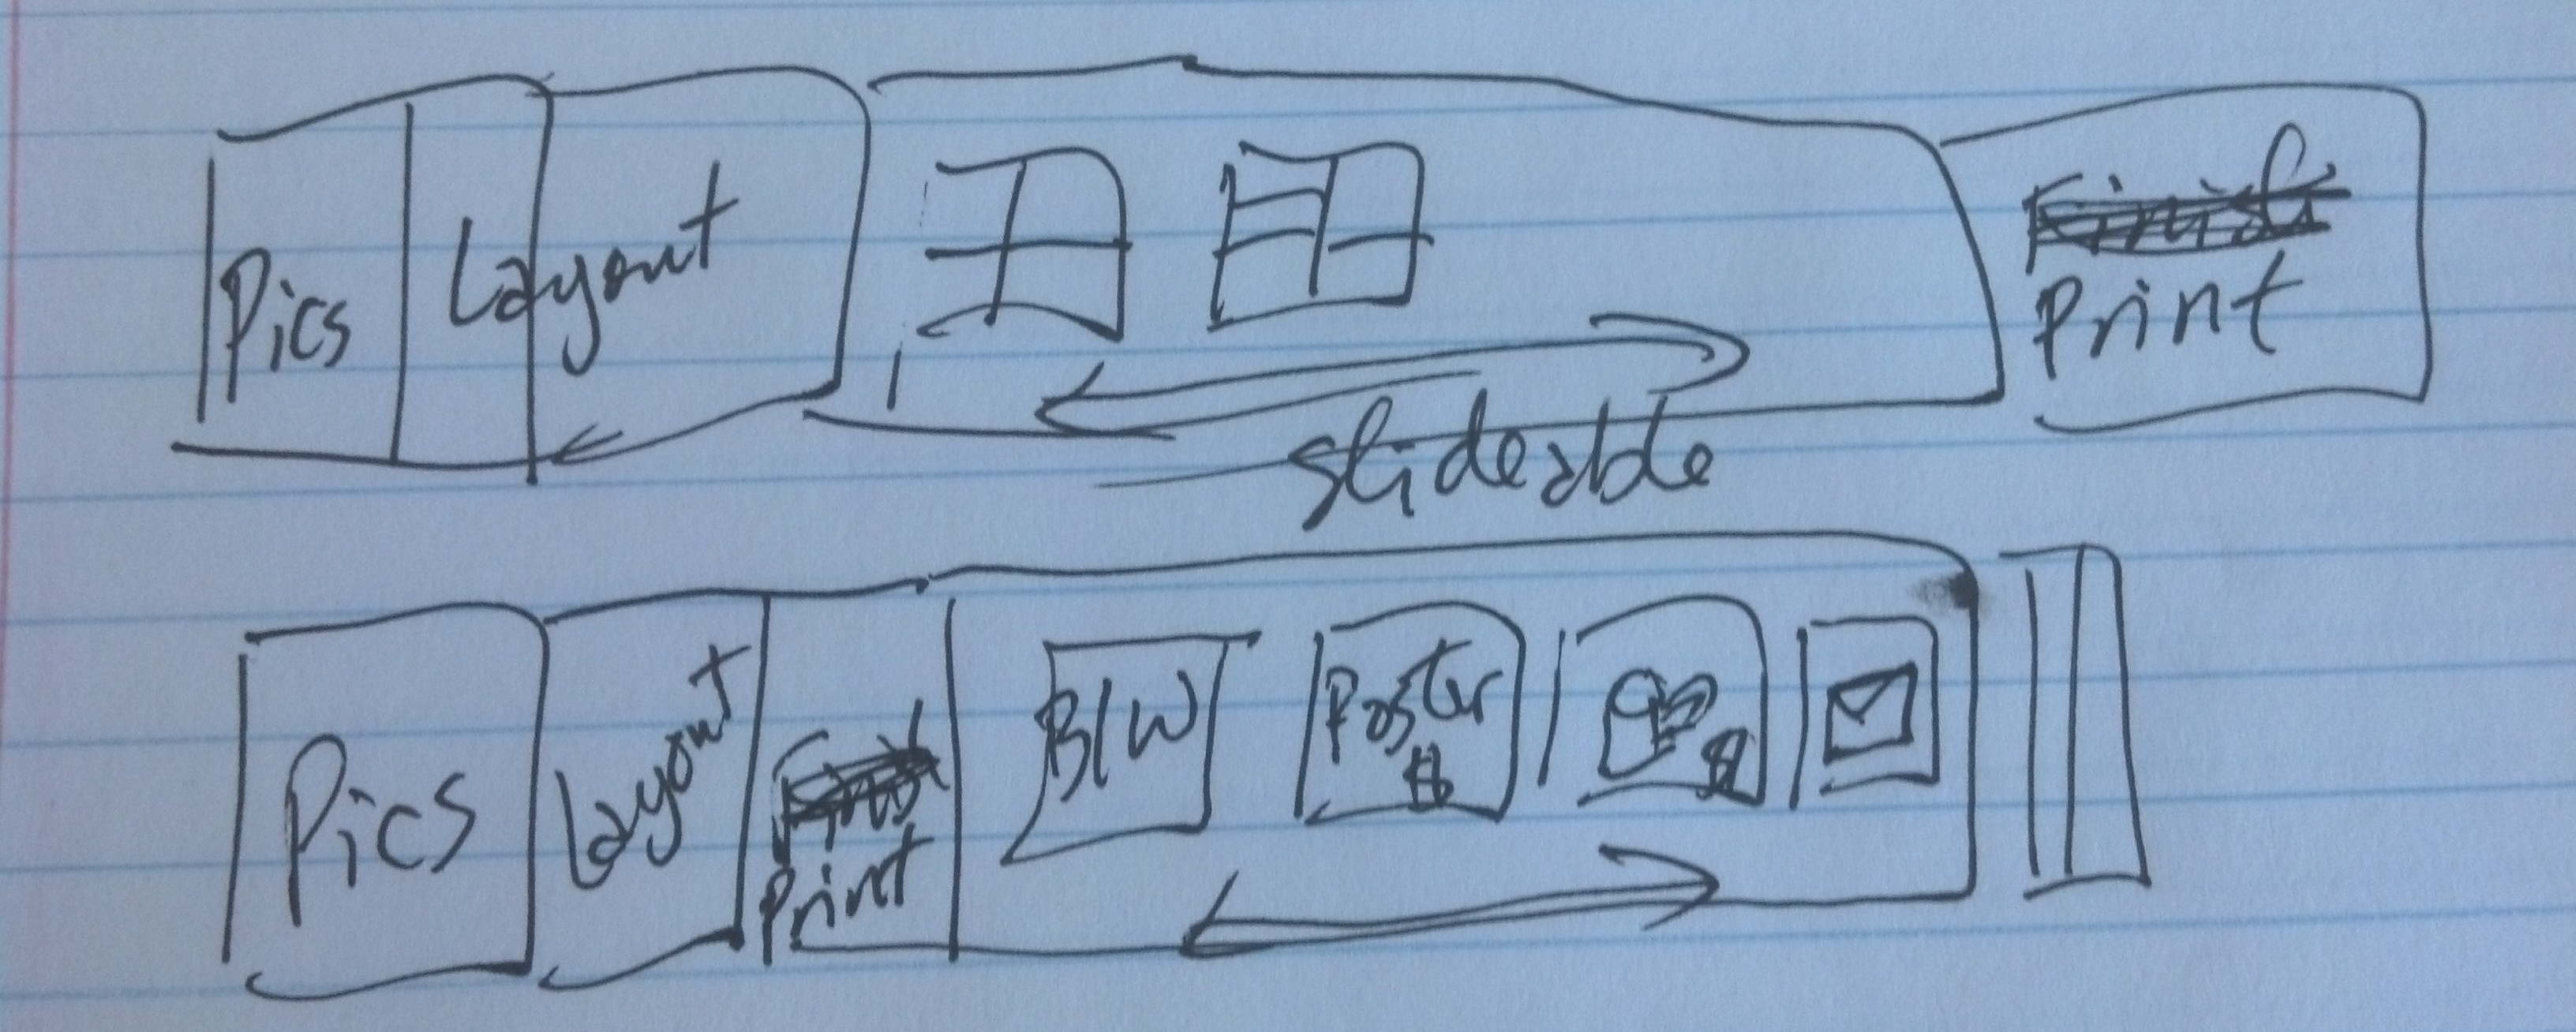
\includegraphics[width=\textwidth, height=120pt]{imgs/titlebar-slider}}
\caption{Design of Sliders for Photo and Layout Browsing}
\label{fig:finalslider}
\end{subfigure}

\caption{Final Prototype Images}
\end{figure*}

\subsection{Personas}

\subsubsection{Teacher - Tom Ryan}
Tom Ryan is a pretty average man who likes to follow rules and tradition for the most part. He is a 4th grade teacher, which can be daunting at times. For Tom, safety is a priority and he does not like to take any chances. Tom has goals for his students. He wants his kids to learn and create sentimental values, but sometimes has to reluctantly put his foot down when engaging the children in order to control small fights over sharing things. 

\subsubsection{Student - Sally Crocker}
A curious little girl, Sally Crocker is an 8 year old 4th grader who sees the world in a very imaginative way. Intimidated by others, she tends to be shy and retract into her introverted personality. Sally just started dance, which is a test of her cautious personality, but finds it very appealing. In all that she does, Sally is a perfectionist and tries to ensure that everything she does is done the right way. Typically, Sally will watch others unless she is alone, where she will won't feel pressured to try something new. She is not a big fan of collaboration, but enjoys doing everything herself and wishes to make her parents proud. 

\subsubsection{Parent - Jan Davis}
Jan Davis is a hard working mother of two kids: a boy of age 12 and a girl of age 5. She loves her kids very much and therefore worries a lot, so Jan is always trying to be sure she is on top of keeping track of her kids. She is always trying to make sure her kids are learning but also having fun; her life revolves a lot around her kids, so her priority is that any family activity is something that they will benefit from. Family values are her core, and she desire to pass them down to her children. 

\subsubsection{General Public - John Q. Public}
John Q. is your typical tourist that intermingles within society in a very private way. He takes pleasure in visiting new places but since heís not very tech savvy, he has to ask a lot of people for guidance. Being a 27 year old, John has a lot of freedom from his indecisive career choices. John does not like to share a lot of his personal life with others either, but he does like to take pictures of his journeys so he can remember them later. 

\subsubsection{Enthusiast - Arty Decker}
Taking pride in all art, including paintings, vintage art, and wacky photographs, Arty Decker is a high end architect that sees the beauty in all of the creations of people. Having a large bank of resources, Arty is a very interested candidate for public venues such as museums, and enjoys scrutinizing their artwork. He also happens to be quite good with a computer and most general electronic or technological devices. Sometimes, however, he seeks advance functionality that doesn't exist. 

\subsubsection{Museum Admin - Marissa Curie}
Marissa Curie has been curator at an art museum for over 11 years and she loves to find new ways of making her museum more productive. Marissa is a poise individual that is very dedicated to her work; in fact it takes up most of her time in life. She is somewhat impatient; therefore, her employees know to get things done when she asks. Very determined to keep her museum in top shape she is always scrutinizing every little thing, even the loose strings on the window drapes. 


%----------------------------------------------------------------------------------------
%	DEVELOP FURTHER
%---------------------------------------------------------------------------------------
\section{Prototype to Continue Further}
The final prototype combines core features from prototypes 1 and 3. Multiple users are supported at once, with the table having split screens; gestural control of photo manipulation is supported. Furthermore, keys are used as well as a smart-phone application to support users taking personal photos to use with the Surface.

The process phase involves two stages. In the first stage, the picture review stage, the user or group brings up their personal library from the visit using a key: the final prototype design of photo selection can be seen in Figure~\ref{fig:finalpic}. The key is placed on top of the Microsoft Surface and the app recognizes the key pattern, associating it with a library in a dictionary data structure. In the next stage, as seen in figure Figure~\ref{fig:finallayout}, the next scene of the app involves layout selection; here, the user(s) select a desired layout of personal photos. The layout and the photos involved can be changed using a layout-selection slider, as seen in Figure~\ref{fig:finalslider}.

Lastly, the user(s) end the session, but before they are given the option to print out photos at the physical store; the print options screen can be seen in Figure~\ref{fig:finalfinish}. Once the requests for prints have been made, an estimate of the time to stop by the store to pick up the print is shown. After a confirmation, the application restarts for new users. The user(s) then can go to the store to pick up their design product; the process continues as new users arrive.

%----------------------------------------------------------------------------------------
%	REDESIGN
%----------------------------------------------------------------------------------------
\section{Re-Design}
%\subsection{Grace}
\textcolor{red}{Type up how we did the redesign and the feedback from class}

%----------------------------------------------------------------------------------------
%	SYSTEM DESIGN DETAILS
%----------------------------------------------------------------------------------------
\section{System Details}
Put text here
\subsection{Interaction Details}
Put text here
\subsection{Architecture Details}
Future section once application is built - elaborate on the user study with the application

%----------------------------------------------------------------------------------------
%	USER EVALUATION
%----------------------------------------------------------------------------------------
\section{User Evaluation}
Put text here
%----------------------------------------------------------------------------------------
%	GESTURE AND INTERACTION EVALUATION
%----------------------------------------------------------------------------------------
\section{Gesture and Interaction Evaluation}
Put text here


%----------------------------------------------------------------------------------------
%	CONCLUSIONS
%----------------------------------------------------------------------------------------
\section{Conclusions}
\subsection{Yongkang}
%Talk about how did good job, summary of findings and design
Tangible design conclusion.

Personas prototype approaches conclusion.

Gesture and action analysis conclusion.

Microsoft surface device conclusion.

Future work.

%----------------------------------------------------------------------------------------
%	APPENDIX - INSTALLATION INSTRUCTIONS
%----------------------------------------------------------------------------------------
\appendix
\section{Installation Instructions}
Put text here


%----------------------------------------------------------------------------------------
%	BIBLIOGRAPHY
%----------------------------------------------------------------------------------------
\bibliographystyle{abbrv}
\bibliography{ArticleDraft}

\end{document}